\chapter{Test}
\section{Linux Kernel Modules}
Kernemodulet er testet ved først at installere modulet ved brug af kommandoen: \textit{sudo insmod simple.ko}.
\\
Modulet skriver til kernel loggen ved initialiseringen. Outputtet fra kernel loggen indhentes ved hjælp af kommandoen dmesg:\\
\textit{dmesg}
\\
\lstinputlisting[language={}]{Testing/Simple.txt}

Modulet slettes derefter ved hjælp af kommmandoen: \textit{sudo rmmod simple}.
\\
\section{Lineær listing}
Kernemodulet for den lineære gennemgang af processer er testet ved at installere modulet ved brug af kommandoen \textit{sudo insmod cumlist.ko}.
\\
Modulet skriver til kernel loggen ved initialiseringen. Outputtet fra kernel loggen indhentes ved hjælp af kommandoen dmesg:\\
\textit{sudo dmesg \textgreater linear.txt}
\\
\\
\subsection{Sammenligning af output}
Resultatet sammenlignes med den indbyggede ps-kommando, med parametrene -el:\\
\textit{ps -el \textgreater pslinear.txt} \\
\\
PS:\\\\
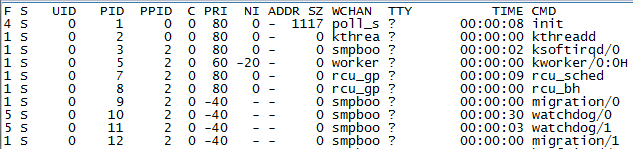
\includegraphics[width=\textwidth]{Testing/PSLinear.png}
\\\\
Implementation:\\\\
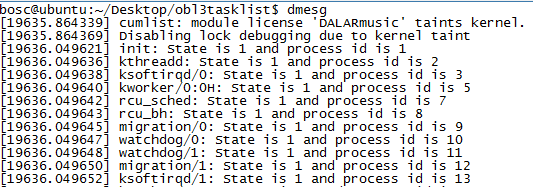
\includegraphics[width=\textwidth]{Testing/Linear.png}
\\\\
Som det kan ses ud fra det udsnit som er taget, så har processerne de samme id i både det implementerede modul og i ps-kommandoen.

\section{DFS listing}
\subsection{Setup}
DFS kernemodulet er testet ved først at registere det med følgende kommando:\\
\textit{sudo insmod dfslist.ko}
\\
\\
Efter som at modulet skriver til kernel loggen ved registrering, er indholdet hentet ud ved at køre kommandoen:\\
\textit{sudo dmesg \textgreater dfs.txt}
\\
\\
Endelig skal resultaterne sammenlignes med den indbyggede ps kommando. Til dette køres følgende kommando for at hente de kørende processer i en træstruktur:\\
\textit{ps axjf \textgreater ps.txt}
\\
\\
Se appendix \ref{ResultaterDFS} for output fra konsollen.

\subsection{Sammenligning af output}
DFS er kendetegnet ved, at første barns børn og børns børn itereres før de resterende børn (og tilsvarende, deres børn og børns børn) fra hovedknuden. Med andre ord forventes det af implementationen, at den udskriver processerne, men inden for hver process itereres ned over processens børn rekursivt og disse udskrives. For eksempel, hvis proceslisten består af process 1 og 2, og disse har børnene 1.1, 1.1.1 og 2.1, skal disse udskrives i rækkefølgen 1, 1.1, 1.1.1, 2, 2.1.\\

Dette viser sig tydeligt at være tilfældet for implementationen, idet processen med process-ID 1053 observeres fra ps.txt:\\
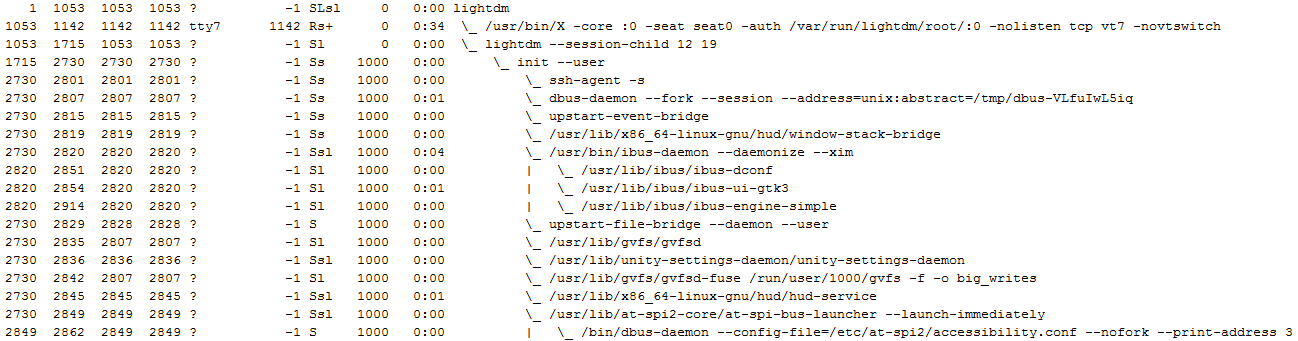
\includegraphics[width=\textwidth]{Testing/DFS1.png}

Her ses det, at process 1053 har en række børn (som også har børn), og af implementationen forventes det derfor, at disse udskrives i rækkefølge. Dette sammenlignes med en del af outputtet fra implementationen:\\
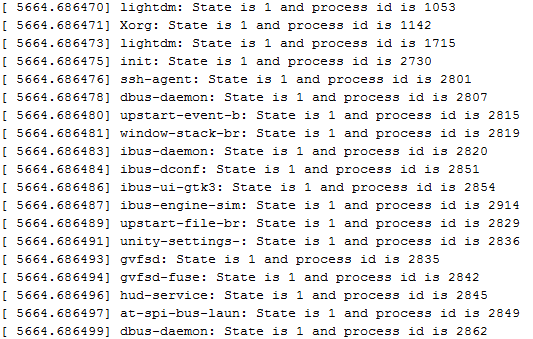
\includegraphics[width=0.6\textwidth]{Testing/DFS2.png}\\
\\
På skærmbilledet ses det, at processerne og deres børn udskrives i rækkefølge - som forventet.